% !TEX root = ../dissertation.tex

\chapter{Geometric Control for Spacecraft}\label{sec:se3_control}

A wide variety of control schemes have been proposed for spacecraft operating around small bodies~\cite{furfaro2013,li2011a}.
In addition, there are a  variety of controllers developed for systems evolving on \( \SE \)~\cite{lee2010,lee2013}.
Much of the previous work has been developed specifically for application on quadrotor aerial vehicles.
In this chapter, we extend their use from quadrotor aerial vehicles into the space domain. 
The geometric control methods used to develop these nonlinear controllers allow for the development of control systems for dynamic systems which evolve on nonlinear manifolds. 
By developing the control system directly on the nonlinear manifold, geometric control techniques provide unique advantages as compared to those developed using local coordinate representations.
Furthermore, the geometric controller avoids the chattering issues inherent in the previous sliding mode control approaches to that have been applied for asteroid landing scenarios.
In addition, rather than offering only a bounded stability guarantee, the proposed nonlinear geometric controller guarantees almost global tracking of the attitude and translational states. 
This stability guarantee is critical for mission operations passing close to the surface over highly irregular terrain.
Furthermore, the coupled geometric controller explicitly considers the attitude coupling of the body in contrast to many of the previous approaches.

This chapter considers the controlled motion of a rigid dumbbell spacecraft about a small body.
We assume that the desired trajectory, \( R_d(t), \vc{x}_d(t) \), are defined as the rotation matrix of the spacecraft body frame with respect to the inertial frame and the relative position of the spacecraft center of mass with respect to the asteorid and defined in the inertial frame, respectively.
In contrast to controllers derived for quadrotor \gls{uav}, the attitude and translational motion are only lightly coupled in the spacecraft scenario.
From the inertial equations of motion given in~\cref{eq:inertial_position_dynamics,eq:inertial_velocity_dynamics,eq:inertial_attitude_dynamics,eq:inertial_angvel_dynamics}, the coupling between the translational and rotational dynamics is due solely to the gravitational moment on the spacecraft.
Furthermore, we assume that we have a fully actuated spacecraft such that we can apply a torque about all three rotational axes and a force in all three directions.
This is in contrast to \glspl{uav} where the system is underactuated and in order to produce certain translational forces the system must first rotate.
This is a relatively standard assumption in the astrodynamics community as most spacecraft contain seperate systems for attitude control, e.g.\ \glspl{rwa}, \glspl{cmg}, or cold gas thrusters, and translational control, e.g.\ cold-gas thrusters, electric propulsion, or large chemical rockets~\cite{hughes2004,wertz1978}.
However, there are also many examples of underactuated spacecraft, such as those with damaged components~\cite{petersen2015a} or cubesats with limited cost and/or size budgets.
In these situations, there are a variety of methods to handle the underactuation, ranging from optimal control techniques, exploiting external forces, or utilizing multiple control loops.

This chapter presents two controllers for the attitude motion and one controller for the translational motion. 
These controllers are computed independently and used to manuever the spacecraft around the small body.
The controllers presented in this section and the low thrust orbital transfer scheme of~\cref{sec:lowthrust_transfers} provide a complete solution for the controlled motion of a spacecraft around a small body.
The reachability based transfers of~\cref{sec:lowthrust_transfers} are ideal for arrival, departure, or other large scale orbital transfers around a small body.
The controllers presented in this chapter are best suited for precise trajectory tracking, such as the shape reconstruction and landing guidance presented in~\cref{sec:shape_reconstruction}.

\section{Control for Attitude Dynamics}\label{sec:attitude_control}

One distinctive feature of the attitude dynamics of rigid bodies is that it evolves on a nonlinear manifold.
The three-dimensional special orthogonal group, or \( \SO \), is the set of \( 3 \times 3 \) orthogonal matrices whose determinant is one.
This configuration space is non-Euclidean and yields unique stability properties which are not observable on a linear space.
For example, it is impossible to achieve global attitude stabilization using continuous time-invariant feedback~\cite{bhat2000}.

Attitude control is typically studied using a variety of attitude parameterizations, such as Euler angles or quaternions~\cite{shuster1993}.
Attitude parameterizations fail to represent the nonlinear configuration space both globally and uniquely~\cite{chaturvedi2011a}.
For example, minimal attitude representations, such as Euler angle sequences or modified Rodriguez parameters, suffer from singularities.
These attitude representations are not suitable for large angular slews.
In order to avoid singularities, the designer must carefully switch the chosen Euler angle sequence based on the operating region.
Another option is to artificially limit the operating region of the rigid body.
This ensures the system operates in a region free from singularities but limits the performance capabilities and ability to perform arbitrarily large angular maneuvers.
Quaternions do not have singularities but they double cover the special orthogonal group.
As a result, any physical attitude is represented by a pair of antipodal quaternions on the three-sphere.
An immediate implication of this ambiguity is that closed-loop stability properties derived using quaternions may not hold for the physical rigid body evolving on the true configuration space, namely the special orthogonal group.
During implementation, the designer must carefully resolve this non-unique representation in quaternion based attitude control systems to avoid undesirable unwinding behavior~\cite{bhat2000}.
This behavior is characterized by situations where the rigid body starts close to the desired attitude, yet the system unnecessarily rotates through a large angle in spite of a small initial error. 

\subsection{Problem Formulation}\label{sec:control_problem_formulation}

In this section, we consider the attitude dynamics of a rigid body, and more specifically those of a dumbbell spacecraft around a small body. 
We consider the inertial attitude dynamics given by~\cref{eq:inertial_attitude_dynamics,eq:inertial_angvel_dynamics} and repeated here as
\begin{align*}
    \dot{\iatt} &= \iatt \iangvel, \\
    J \dot{\iangvel} + \hat{\iangvel} J \iangvel &= M_{ext} + u_m,
\end{align*}
where we combined the gravitational moment into a single term \( M_{ext} \in \R^3 \) which defines the total external moment on the spacecraft.
The control system developed in this section are focused on the inertial motion of the spacecraft.
The same control system can also be applied to the relative equations of motion defined in~\cref{sec:asteroid_dumbbell_eoms} by using the relative variables.

The first step in designing a control system on a nonlinear manifold \( \Q \) is the selection of a proper configuration error function. 
This configuration error function, \( \Psi : \Q \times \Q \to \R \), is a smooth and proper positive definite function that measures the error between the current configuration and a desired configuration. 
Once an appropriate configuration error function is chosen, one can then define a configuration error vector and a velocity error vector in the tangent space \( \mathsf{T}_q \Q \) through the derivatives of \( \Psi \)~\cite{bullo2004}. 
With the configuration error function and vectors, the remaining procedure is analogous to nonlinear control design on Euclidean vector spaces. 
One chooses control inputs as functions of the state through a Lyapunov analysis on \Q.
The configuration error function used in this analysis has been used in~\cite{bullo2004,chaturvedi2009,lee2011a,kulumani2017a}.
In this section we summarize the properties developed previously and present several extensions for our use in the case of motion around an asteroid.

% trackign control
In order to determine the attitude control input, we first define a desired attitude tracking command.
An arbitrary smooth attitude tracking command \( R_d (t) \in \SO \) is given as a function of time.
% TODO Add link to this equation in dynamic derivation
The corresponding angular velocity command is obtained using the attitude kinematics equation, \( \hat{\Omega}_d = R_d^T \dot{R}_d \).
With the desired attitude command, \( R_d(t), \Omega_d(t) \), we then define the errors associated with the attitude and angular velocity.
The attitude and angular velocity tracking errors must be careful chosen to remain on the tangent bundle of \(\SO\).
The control objective is then to determine a control input \( u_m \) such that the system is able to accurately track the attitude command \( R_d(t) \) and compensate for the external moment \( M_{ext} \).

\begin{prop}[ Attitude Configuration Error Function ]\label{prop:attitude_control_configuration_error}

First, an attitude error function \(A : \SO \times \SO  \to \R \), an attitude error vector \( e_R : \SO \times \SO \to \R \), and an angular velocity error \( e_\Omega : \SO \times \R^3 \times \SO \times \R^3 \) are defined as
\begin{subequations}\label{eq:attitude_error_function}
\begin{align}
    A(R, R_d) &= \frac{1}{2}  \tr{G\parenth{I - R_d^T R}}, \label{eq:A} \\
    e_R &= \frac{1}{2} G \parenth{R_d^T R - R^T R_d^\vee}, \label{eq:eRA}\\
    e_\Omega &= \Omega - R^T R_d \Omega_d \label{eq:eWA}.
\end{align}
\end{subequations}
Then the following properties hold:
\begin{enumerate}
    \item \label{item:prop_A_psd} \( A \) is locally positive definite about \( R = R_d \) on \( \SO \).
    \item \label{item:prop_eRA} The variation of \( A \) with respect to a variation of \( \delta R = R \hat{\eta} \) for \( \eta \in \R^3 \) is given by
	\begin{align}\label{eq:dirDiff_A}
		\dirDiff{A}{R} &= \eta \cdot e_{R} ,
	\end{align}
	where the notation \( \dirDiff{A}{R} \) represents the directional derivative of $A$ with respect to $R$ along the direction $\delta R$.
\item \label{item:prop_A_critical_points} The critical points of \( A \), where \( e_R = 0 \) are \( \braces{R_d} \cup \braces{R_d \exp(\pi \hat s) } \) for \( s \in \braces{e_1, e_2, e_3}\)
    \item \label{item:prop_A_quadratic} \( \Psi \) is a locally quadratic function, which means there exist constants \( 0 < n_1 \leq n_2 \) such that
    \begin{align}\label{eq:A_bound}
        n_1 \norm{e_R}^2 \leq \Psi(R) \leq n_2 \norm{e_R}^2 ,
    \end{align}
    for $0<\psi < h_1 $ where the constants \( n_1 = \frac{h_1}{h_2 + h_3} \) and \( n_2 = \frac{h_1 h_4}{h_5 \parenth{h1 - \psi} }\) for
	\begin{align*}
		h_1 &= \min\braces{g_1 + g_2, g_2 + g_3 , g_3 + g_1} ,\\
		h_2 &= \max\braces{\parenth{g_1 -g_2}^2,\parenth{g_2 -g_3}^2 , \parenth{g_3 -g_1}^2} ,\\
		h_3 &= \max\braces{\parenth{g_1 + g_2}^2, \parenth{g_2 + g_3}^2 , \parenth{g_3 + g_1}^2}, \\		
        h_4 &= \max\braces{g_1 + g_, g_2 +g_3, g_3 + g_1}, \\
        h_5 &= \max\braces{\parenth{g_1 + g_2}^2, \parenth{g_2 + g_3}^2, \parenth{g_3 + g_1}^2}.
	\end{align*}
\end{enumerate}
\end{prop}
\begin{proof}
    See~\Cref{proof:attitude_config_error}
\end{proof}

With the appropriate attitude configuration error we now present the error dynamics in~\cref{prop:attractive_error_dynamics}, which are used in the subsequent development of the nonlinear control system.
\begin{prop}\label{prop:attractive_error_dynamics}
    The attitude error dynamics for \( A(R, R_d), e_\Omega \) satisfy
	\begin{gather}
    	\diff{}{t} \parenth{A(R)} = e_{R_A} \cdot e_\Omega , \label{eq:A_dot} \\
		\diff{}{t} \parenth{e_{R_A}} = E(R, R_d) e_\Omega , \label{eq:eRA_dot} \\
        \diff{}{t} \parenth{e_\Omega} = J^{-1} \parenth{-\hat{\Omega} J \Omega + u_m + M_{ext}} , \label{eq:eW_dot}
	\end{gather}
	where the matrix \(E(R,R_d)\in \R^{3\times3} \) is given by
	\begin{align}
		E(R,R_d) = &\frac{1}{2} \parenth{\tr{R^T R_d G}I - R^T R_d G} , \label{eq:E} \\
	\end{align}
\end{prop}
\begin{proof}
    See~\Cref{proof:attractive_error_dynamics}
\end{proof}

With the appropriate attitude configuration error we now present an attitude controller for attitude stabilization and tracking of the inertial attitude dynamics given in~\cref{eq:inertial_attitude_dynamics,eq:inertial_angvel_dynamics}.

\begin{prop}[Control for Attitude Dynamics]\label{prop:att_control}
	Given a desired attitude command \( \parenth{R_d, \Omega_d = 0} \) and positive constants \( k_R, k_\Omega \in \R \) we define a control input \( u \in \R^3 \) as follows
	\begin{gather}
        u = -k_R e_R - k_\Omega e_\Omega + \Omega \times J \Omega - M_{ext}. \label{eqn:nodist_control}
	\end{gather}
	Then the zero equilibrium of the attitude error is asymptotically stable.
\end{prop}
\begin{proof}
See~\Cref{proof:att_control}
\end{proof}

\section{Adaptive Attitude Control with State Inequality Constraints}\label{sec:constrained_attitude_control}

Many physical rigid body systems must perform large angular slews in the presence of state constraints.
For example, autonomous spacecraft or aerial systems are typically equipped with sensitive optical payloads, such as infrared or interferometric sensors.
These systems require retargeting while avoiding direct exposure to sunlight or other bright objects.
In addition, many ground based attitude testing environments, such as air bearing platforms, must operate in the presence of physical obstructions.
Determining a satisfactory attitude control maneuver in the presence of state constraints is a challenging task.
The removal of constrained regions from the rotational configuration space results in a \textit{nonconvex} region.
The attitude control problem in the feasible configuration space has been extensively studied~\cite{bullo2004,mayhew2011,lee2015}.
However, the attitude control problem in the presence of constraints has received much less attention.

% discuss how previous papers (mcinnes and lee/meshabi) have short comings
Several approaches have been developed to treat the attitude control problem in the presence of constraints.
A conceptually straightforward approach is used in~\cite{hablani1999} to determine feasible attitude trajectories prior to implementation.
The algorithm determines an intermediate point such that an unconstrained maneuver can be calculated for each subsegment.
Typically, an optimal or easily implementable on-board control scheme for attitude maneuvers is applied to maneuver the vehicle along these segments.
In this manner, it is possible to solve the constrained attitude control problem by linking several intermediary unconstrained maneuvers.
While this method is conceptually simple, it is difficult to generalize for an arbitrary number of constraints.
In addition, this approach is only applicable to problems where the selection of intermediate points are computationally feasible.

The approach in~\cite{frazzoli2001} involves the use of randomized motion planning algorithms to solve the constrained attitude control problem.
A graph is generated consisting of vertices from an initial attitude to a desired attitude. 
A random iterative search is conducted to determine a path through a directed graph such that a given cost, which parameterizes the path cost, is minimized.
The random search approach can only stochastically guarantee attitude convergence as it can be shown that as the number of vertices in the graph grow, the probability of nonconvergence goes to zero.
However, the computational demand grows as the size of the graph is increased and a new graph is required when constraints are modified. 
As a result, random search approaches are ill-suited to on-board implementation or in scenarios that require agile maneuvers.

Model predictive control for spacecraft attitude dynamics is another popular approach and has been studied in~\cite{guiggiani2014,kalabic2014,gupta2015}.
These methods rely on linear or non-linear state dynamics to repeatedly solve a finite-time optimal control problem.
Also known as receding horizon control, the optimal control formulation allows for a straight forward method to incorporate state and control constraints.
Computing the optimal control strategy over a moving horizon allows for a form of feedback type control rather than the more typical open-loop optimal control solution.
Due to the iterative nature of solving optimization problems, model predictive control methods are computational expensive and frequently apply direct optimization methods to solve the necessary conditions for optimality.
Therefore, these methods are complicated to implement and may not be suitable for real-time control applications.
  
% Previous potential function approach - developed using attitude parameterizations - singularities/ambiguities
Artificial potential functions are commonly used to handle kinematic constraints for a wide range of problems in robotics~\cite{rimon1992}.
The goal is the design of attractive and repulsive terms which drive the system toward or away from a certain obstacle, respectively.
The attractive function is designed to drive the system towards the desired state.
Similarly, a repulsive function is constructed such that the system is directed away from the constraints. 
The superposition of these functions allows one to apply standard feedback control schemes for stabilization and tracking.
More specifically, artificial potential functions have previously been applied to the spacecraft attitude control problem in~\cite{lee2011b,mcinnes1994}.
However, both of these approaches were developed using attitude parameterizations, namely Euler angles and quaternions, and as such, they are limited by the singularities of minimal representations or the ambiguity of quaternions.

This section is focused on developing an adaptive attitude control scheme in the presence of attitude inequality constraints on \(\SO\).
We apply a potential function based approach developed directly on the nonlinear manifold \(\SO\). 
By characterizing the attitude both globally and uniquely on \(\SO\), our approach avoids the issues of attitude parameterizations, such as kinematic singularities and ambiguities, and is geometrically exact. 
A configuration error function on \(\SO\) with a logarithmic barrier function is proposed to avoid constrained regions. 
Instead of calculating a priori trajectories, as in the randomized approaches, our approach results in a closed-loop attitude control system. 
This makes it ideal for on-board implementation on UAV or spacecraft systems. 
In addition, unlike previous approaches our control system can handle an arbitrary number of constrained regions without modification.
This approach results in a conceptually simple obstacle avoidance scheme which extends the previous work of artificial potential functions on Euclidean spaces to the special orthogonal group.
Furthermore, we use this new configuration error function to design an adaptive update law to enable attitude convergence in the presence of uncertain disturbances. 

\paragraph{State Inequality Constraint}\label{sec:state_inequality_constraint}
The two-sphere is the manifold of unit-vectors in \( \R^3 \), i.e., \( \Sph^2 = \{ q \in \R^3 \,  \vert \, \norm{q} = 1 \}\).
We define \( r \in \Sph^2 \) to be a unit vector from the mass center of the rigid body along a certain direction and it is represented with respect to the body-fixed frame.
For example, \( r \) may represent the pointing direction of an on-board optical sensor.
We define \( v \in \Sph^2 \) to be a unit vector from the mass center of the rigid body toward an undesired pointing direction and represented in the inertial reference frame.
For example, \( v \) may represent the inertial direction of a bright celestial object or the incoming direction of particles or other debris.
It is further assumed that optical sensor has a strict non-exposure constraint with respect to the celestial object.
We formulate this hard constraint as
\begin{align}
	r^T R^T v \leq \cos \theta , \label{eqn:constraint}
\end{align}
where we assume \( \ang{0} \leq \theta \leq \ang{90}  \) is the required minimum angular separation between \( r \) and \( R^T v \). 
The objective is to a determine a control input \( u \) that stabilizes the system from an initial attitude \( R_0 \) to a desired attitude \( R_d \) while ensuring that~\cref{eqn:constraint} is always satisfied.

\paragraph{Constrained Attitude Error Function}
To handle the attitude inequality constraint, we propose a new attitude configuration error function. 
More explicitly, we extend the trace form used in~\cite{bullo2004,lee2013b,kulumani2017a} and presented in~\Cref{prop:attitude_control_configuration_error} for attitude control on \(\SO\) with the addition of a logarithmic barrier function. 
Based on the proposed configuration error function, a nonlinear geometric attitude controller is constructed. 
A smooth control system is first developed assuming that there is  no disturbance, and then it is extended to include an adaptive update law for stabilization in the presence of unknown disturbances. 
The proposed attitude configuration error function and several properties are summarized as follows.
\begin{prop}[Constrained Attitude Error Function] \label{prop:repulsive_configuration_error}
Define an attitude error function \( \Psi : \SO \to \R \), an attitude error vector \( e_R \in \R^3 \), and an angular velocity error vector \( e_\Omega \in \R^3 \) as follows:
\begin{gather}
	\Psi(R, R_d) = A(R, R_d) B(R) , \label{eq:psi} \\
	e_R = e_{R_A} B(R) + A(R,R_d) e_{R_B} , \label{eq:eR} \\
	e_\Omega = \Omega , \label{eq:eW}
\end{gather}
with
\begin{gather}
	B(R) = 1 - \frac{1}{\alpha} \ln \left( \frac{\cos \theta -  r^T R^T v}{1 + \cos \theta}\right). \label{eq:B} \\
	e_{R_B} = \frac{\left( R^T v\right)^\wedge r}{\alpha \left(r^T R^T v - \cos \theta \right)}. \label{eq:eRB} 
\end{gather}	
where \( \alpha \in \R \) is defined as a positive constant.
Then, the following properties hold
\begin{enumerate}
	\item \label{item:prop_psi_psd} \(\Psi\) is positive definite about \( R = R_d\) on $\SO$.
	\item \label{item:prop_erb} The variation of \( B(R) \) with respect to a variation of \( \delta R = R \hat{\eta} \) for \( \eta \in \R^3 \) is given by
	\begin{align}\label{eq:dirDiff_B}
		\dirDiff{B}{R} &= \eta \cdot e_{R_{B}}.
	\end{align}
    \item \label{item:prop_psi_quadratic} \( \Psi \) is a locally quadratic function, which means there exist constants \( 0 < n_1 \leq n_2 \) such that
    \begin{align}\label{eq:psi_bound}
        n_1 \norm{e_R}^2 \leq \Psi(R) \leq n_2 \norm{e_R}^2 ,
    \end{align}
    on the neighborhood $D$ of the desired attitude \( R_d \)
    \begin{align}\label{eq:psi_quadratic_domain}
        D = \braces{R\in\SO  \vert \Psi < \psi < h_1, r^T R^T v < \beta < \cos \theta}
    \end{align}
    for $0<\psi < h_1 $ and $0< \beta<\cos\theta$. 
\end{enumerate}
\end{prop}
\begin{proof}
    See~\Cref{proof:repulsive_configuration_error}
\end{proof}

\Cref{eq:psi} is composed of an attractive term, \( A (R) \) toward the desired attitude, and a repulsive term, \( B(R) \) away from the undesired direction \( R^T v \).
In order to visualize the attitude error function on \( \SO \), we utilize a spherical coordinate representation.
Recall, that the spherical coordinate system represents the position of a point relative to an origin in terms of a radial distance, azimuth, and elevation.
This coordinate system is commonly used to define locations on the Earth in terms of a latitude and longitude.
Similarly, the positions of celestial objects are defined on the celestial sphere in terms of right ascension and declination. 
\begin{figure}[htbp]%
    \centering 
    \subcaptionbox{Attractive attitude error function \( A(R) \) in spherical coordinate representation.\label{fig:attract_error} }{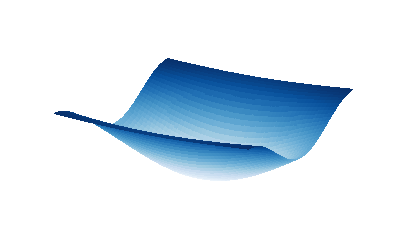
\includegraphics[trim={8mm 2mm 8mm 2mm}, clip, width=0.49\textwidth]{figures/2016_IJCAS/attract_error.pdf}}~%
    \subcaptionbox{Repulsive attitude error function \( B(R) \) spherical coordinate representation.\label{fig:avoid_error} }{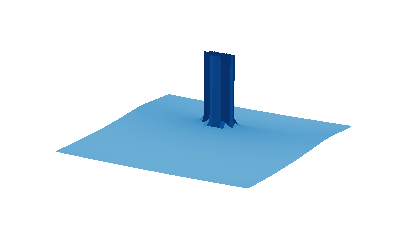
\includegraphics[trim={8mm 2mm 8mm 2mm}, clip, width=0.49\textwidth]{figures/2016_IJCAS/avoid_error.pdf}}%

    \subcaptionbox{Combined attitude error function \( \Psi \) composed as the product of \( A(R) \) and \( B(R) \).\label{fig:combined_error} }{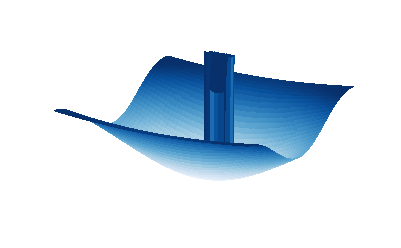
\includegraphics[trim={8mm 2mm 8mm 2mm}, clip, width=0.49\textwidth]{figures/2016_IJCAS/combined_error.pdf}}%
    \caption{Visualization of Configuration Error Functions using spherical coordinate representation. 
    The horizontal axes are representative of angles on the sphere.
    The height of the surface denotes the value of the error function.
    The minimum is located at the desired attitude \( R_d \) while the regions around obstacles have large error values.}
    \label{fig:config_error} 
\end{figure}%
We apply this concept and parameterize the rotation matrix \( R \in \SO \) in terms of the spherical angles \( \SI{-180}{\degree} \leq \lambda \leq \SI{180}{\degree}  \) and \( \SI{-90}{\degree} \leq \beta \leq \SI{90}{\degree} \). 
Using the elementary Euler rotations, the rotation matrix is now defined as \( R = \exp( \lambda \hat{e}_2) \exp( \beta \hat{e}_3) \).
We iterate over the domains of \( \lambda\) and \(\beta\) in order to rotate the body-fixed vector \( r \) throughout the two-sphere \( \S^2 \).
Applying this method,~\cref{fig:config_error} allows us to visualize the error function on \( \SO \).
The horizontal axes of~\cref{fig:config_error} represent the domain of the spherical angles \( \lambda \) and \( \beta \) in degrees, while the vertical axes represent the unitless magnitude of the error functions defined in~\cref{eq:psi,eq:A,eq:B}.
The attractive error function, given by~\cref{eq:A}, has been previously used for attitude control on \(\SO\).
The potential well of \( A(R)\) is illustrated in~\cref{fig:attract_error}, where the desired attitude lies at the minimum of \( A(R) \).

To incorporate the state inequality constraints we apply a logarithmic barrier term.
Barrier functions are typically used in optimal control and motion planning applications.
A visualization of the repulsive error function is presented in~\cref{fig:avoid_error} which shows that as the boundary of the constraint is neared, or \( r^T R^T v \to \cos \theta \), the barrier term increases, \( B \to \infty\).
We use the scale factor~\(\frac{1}{1+\cos \theta} \) to ensure that \( \Psi \) remains positive definite.
The logarithmic function is popular as it quickly decays away from the constraint boundary.
The positive constant \( \alpha \) serves to shape the barrier function.
As \( \alpha \) is increased the impact of \( B(R) \) is reduced away from the constraint boundary. 
The superposition of the attractive and repulsive functions is shown in~\cref{fig:combined_error}.
The control system is defined such that the attitude trajectory follows the negative gradient of \( \Psi \) toward the minimum at \( R = R_d \), while avoiding the constrained region.

While~\cref{eq:B} represents a single inequality constraint given as~\cref{eqn:constraint}, it is readily generalized to multiple constraints of an arbitrary orientation. 
For example, the configuration error function can be formulated as $\Psi=A[1+\sum_i C_i]$, where $C_i$ has the form of $C_i=B-1$ for the $i$-th constraint. 
In this manner, one may enforce multiple state inequality constraints, and we later demonstrate this through numerical simulation. 
This is in contrast to many previous approaches which are computationally difficult to extend to situations with multiple constraints.
We present the dynamics of the combined configuration error function in~\Cref{prop:repulsive_error_dynamics}, which are used in the subsequent development of the nonlinear control system.

\begin{prop}[Constrained Error Dynamics]\label{prop:repulsive_error_dynamics}
	The attitude error dynamics for \( \Psi, e_R, e_\Omega \) satisfy 
	\begin{gather}
		\diff{}{t} \parenth{\Psi} = e_R \cdot e_\Omega , \label{eq:psi_dot}\\
		\diff{}{t} \parenth{e_R} = \dot{e}_{R_A} B + e_{R_A} \dot{B} + \dot{A}e_{R_B} + A \dot{e}_{R_B} , \label{eq:eR_dot} \\
		\diff{}{t} \parenth{e_{R_B}} = F(R) e_\Omega , \label{eq:eRB_dot} \\
		\diff{}{t} \parenth{B(R)} = e_{R_B} \cdot e_\Omega , \label{eq:B_dot}
	\end{gather}
	where the matrix \(F(R) \in \R^{3\times3} \) is given by
	\begin{align}
		F(R) = &\frac{1}{\alpha \parenth{r^T R^T v - \cos \theta}} \left[\parenth{v^T R r} I - R^T v r^T + \frac{R^T \hat{v} R r v^T R \hat{r}}{\parenth{r^T R^T v - \cos \theta}}\right]. \label{eq:F}
	\end{align}
\end{prop}
\begin{proof}
    See~\Cref{proof:repulsive_error_dynamics}.
\end{proof}

We extend the results of the controller presented in~\cref{prop:att_control} with the addition of a fixed but unknown disturbance \( W(R, \Omega) \Delta \).
Consider the attitude dynamics with an additional disturbance moment as
\begin{align}
    J \dot{\iangvel} + \hat{\iangvel} J \iangvel &= W(R, \Omega)\Delta  +  M_{ext} + u_m,\label{eq:Wdot}
\end{align}
where \( W(R, \Omega) : \SO \times \R^3 \to \R^{3 \times p } \) is a known function of the attitude and angular velocity.
The disturbance is represented by \( \Delta \in \R^p \) and is an unknown but fixed uncertain parameter.
We also assume that a bound on \( W(R, \Omega) \) and \( \Delta \) is known and given by
\begin{align}\label{eq:disturbance_bounds}
    \norm{W} \leq B_W, \quad \norm{\Delta} \leq B_\Delta,
\end{align}
for positive constants \(B_W, B_\Delta\).
This force of uncertainty enters the system dynamics through the input channel and as a result is referred to as a matched uncertainty.
While this form of uncertainty is easier than the unmatched variety, many physically realizable disturbances may be modeled in this manner.
For example, orbital spacecraft are subject to gravity gradient torques, such as the dumbbell spacecraft model considered in this dissertation.
Another terrestrial example is frequently encountered by unmanned aerial vehicles.
Multiple actuator systems, such as quadrotor aerial vehicles, may exhibit an uneven mass distribution during load transportation or must operate in the presence of turbulence.
An adaptive control system is introduced to asymptotically stabilize the system to a desired attitude while ensuring that state constraints are satisfied. %We first show several properties of the controlled system. 

\begin{prop}[Bound on \( \dot{\vc{e}}_R \)]\label{prop:eR_dot_bound}
Consider the neighborhood \( D \), given in~\cref{prop:repulsive_configuration_error}, about the desired attitude, then the following statements hold:
\begin{enumerate}
    \item \label{item:prop_eR_dot_bound_AB} Upper bounds of \( A(R) \) and \( B(R) \) are given by
        \begin{gather}
            \norm{A} < b_2 \norm{e_{R_A}}^2 < c_A  , \quad \norm{B} < c_B. \label{eqn:AB_bound}
        \end{gather}
        where the constant \( b_2\) is given by \( b_2 = \frac{h_1 h_4}{h_5 \parenth{h_1 - \psi}}\) for
        \begin{align*}
            h_4 &= \min\braces{g_1 + g_2, g_2 + g_3 , g_3 + g_1} ,\\
            h_5 &= \min\braces{\parenth{g_1 + g_2}^2,\parenth{g_2 + g_3}^2 , \parenth{g_3 + g_1}^2}.
        \end{align*}
    \item \label{item:prop_eR_dot_bound_EF} Upper bounds of \( E(R,R_d) \) and \( F(R) \) are given by
        \begin{gather}
            \norm{E} \leq \frac{1}{\sqrt{2}} \tr{G}  , \label{eqn:E_bound} \\
            \norm{F} \leq \frac{\parenth{\beta^2 + 1}\parenth{\beta - \cos \theta}^2 + 1 + \beta^2 \parenth{\beta^2-2}}{\alpha^2 \parenth{\beta-\cos \theta}^4}. \label{eqn:F_bound}
        \end{gather}
    \item Upper bounds of the attitude error vectors \( e_{R_A} \) and \( e_{R_B} \) are given by
        \begin{gather}
            \norm{e_{R_A}} \leq \sqrt{\frac{\psi}{b_1}}, \label{eqn:eRA_bound} \\
            \norm{e_{R_B}} \leq \frac{\sin\theta}{\alpha \parenth{\cos \theta - \beta}}. \label{eqn:eRB_bound}
        \end{gather}
\end{enumerate}
These results are combined to yield a maximum upper bound of the time derivative of the attitude error vector \( \dot{e}_R \) as
\begin{gather}
	\norm{\dot{e}_R} \leq H \norm{e_\Omega} ,\label{eqn:eR_bound}
\end{gather}
where  \( H \in \R \) is defined as
\begin{gather}
	H = \norm{B} \norm{E} + 2 \norm{e_{R_A}} \norm{e_{R_B}} + \norm{A}\norm{F}. \label{eqn:H}
\end{gather}
\end{prop}
\begin{proof}
See~\Cref{proof:eR_dot_bound}
\end{proof}

Adaptive control is typically used in dynamical systems with varying or uncertain components.
In~\Cref{prop:adaptive_control}, we present an adaptive attitude controller which handles uncertain disturbances while satisfying the state inequality constraints.
\begin{prop}[Constrained Adaptive Attitude Control]\label{prop:adaptive_control}
Given  a desired attitude command \( (R_d, \Omega_d = 0 )\) and positive constants \( k_R, k_\Omega, k_\Delta, c \in \R \), we define a control input \( u \in \R^3\) and an adaptive update law for the estimated uncertainty \( \bar{\Delta} \) as follows:
\begin{align}
    u &= - k_R e_R - k_\Omega e_\Omega + \Omega \times J \Omega - W \bar{\Delta} - M_{ext} , \label{eqn:adaptive_control} \\
	\dot{\bar{\Delta}} &= k_\Delta W^T \parenth{e_\Omega + c e_R}. \label{eqn:delta_dot}
\end{align}
If \( c \) is chosen such that
\begin{gather}
	0 < c < \min \braces{\sqrt{\frac{2 \lambda_m k_R n_1}{\lambda_M^2}},
	%\sqrt{\frac{2 k_R n_2}{\lambda_M}}, 
	\frac{4 k_R k_\Omega}{k_\Omega^2 + 4 k_R \lambda_M H}} , \label{eqn:c_bound}
\end{gather}
  the zero equilibrium of the error vectors is stable in the sense of Lyapunov. Furthermore, $e_R,e_\Omega\rightarrow 0$ as $t\rightarrow\infty$, and $\bar\Delta$ is  bounded.
\end{prop}
\begin{proof}
See~\Cref{proof:adaptive_control}
\end{proof}

Nonlinear adaptive controllers have been developed for attitude stabilization in terms of modified Rodriguez parameters and quaternions, as well as attitude tracking in terms of Euler angles. 
The proposed control system is developed on \(\SO\) and avoids the singularities of Euler angles and Rodriguez parameters while incorporating state inequality constraints. 
In addition, the unwinding and double coverage ambiguity of quaternions are also completely avoided. 
The control system handles uncertain disturbances while avoiding constrained regions.

Compared to the previous work on constrained attitude control, we present a geometrically exact control system without parameterizations.
The controller is designed on the true configuration manifold, \( \SO \), and is free from the issues associated with other attitude representations.
In addition, we incorporate state inequality constraints for the first time on \( \SO \).
The presented control system is computed in real-time and offers significant computational advantages over previous iterative methods. 
In addition, the rigorous mathematical proof guarantees stability.
This is in contrast to many of the previous methods which offer no stability guarantees.
The presented analysis offers provable bounds on the expected motion, which are critical for hardware implementation or mission critical applications.

\section{Control for Translational Dynamics}

In order to fully control the spacecraft, we require an additional translational controller.
In the case of missions about very small bodies, typical orbital transfer and control schemes become impractical as the gravitational attraction is too weak to enable proper Keplerian orbits~\cite{broschart2005}.
Furthermore, since the gravitational attraction is very small in magnitude the effect of external disturbances, such as solar radiation pressure or differential forces on the body, become much more significant.
In particular, various approaches have been developed for closed-loop control near small-bodies.
For example, researchers have developed hovering type schemes~\cite{broschart2005,sawai2002}, sliding mode based approaches for landing~\cite{furfaro2013,liaw2000,zexu2012}, optimal control~\cite{guelman1994,guo2011,lantoine2006,miso1999}, and most recently geometric control~\cite{kulumani2017b,misra2015a}.
In this section, we present and derive a closed loop control scheme for the translational position of a spacecraft around a small body.
The method applies standard nonlinear control techniques for systems on Euclidean spaces~\cite{khalil1996}.

\paragraph{Problem Formulation}\label{sec:translation_control_problem_formulation}

We consider the translational dynamics of a rigid spacecraft around a small body.
The inertial translational dynamics were defined in~\cref{sec:inertial_dumbbell_eoms} and are given as
\begin{align*}
    \dot{\ipos} &= \ivel,\\
    m \dot{\ivel} &= F_{ext} + u_f,
\end{align*}
where \( m \in \R^1 \) is the total mass of the spacecraft and \( F_{ext} \in \R^3 \) is defined as the sum of the total external force on the vehicle.
With the inertial dynamics, the goal of the controller is to determine a control input \( u_f \in \R^3 \) such that the spacecraft accurately follows a desired trajectory \( x_d(t) \in \R^3 \).

First, we define a smooth tracking command \( x_d(t) \in \R^3 \), which defines the desired position of the spacecraft in the inertial frame.
The tracking error vectors are easier to define as they evolve on a Euclidean space rather than a nonlinear manifold and are given by
\begin{subequations}\label{eq:translation_error_variables}
\begin{align}
    e_x &= x - x_d ,\\
    e_v &= v - \dot{x}_d.
\end{align}
\end{subequations}
The error dynamics are given by
\begin{subequations}\label{eq:translation_error_dynamics}
\begin{align}
    \dot{e}_x &= v - \dot{x}_d, \\
    \dot{e}_v &= \dot{v} - \ddot{x}_d .
\end{align}
\end{subequations}
A control input, \( u_f \), is derived to ensure asymptotic trajectory tracking for the translational dynamics.
\begin{prop}[Control for Translation Dynamics]\label{prop:translational_control}
    Given a desired trajectory \( \vc{x}_d \) and positive constants \( k_x, k_v, c \in \R \) we define a control input \( \vc{u}_f \in \R \) as follows:
    \begin{align}\label{eq:translational_control}
        \vc{u}_f = -k_x e_x - k_v e_v - F_{ext} + m \ddot{x}_d .
    \end{align}
    If \( c \) is chosen such that
    \begin{align}\label{eq:translational_control_gain_bound}
        0 < c < \min \braces{\sqrt{k_x m}, \frac{4 k_x k_v m}{ k_v \parenth{4 k_x m - k_v} }   }
    \end{align}
    then the zero equilibrium of the error vectors~\cref{eq:translation_error_variables} is stable in the sense of Lyapunov.
    Furthermore, \( e_x, e_v \to 0 \) as \( t \to \infty\).
\end{prop}
\begin{proof}
    See~\cref{proof:translational_control}
\end{proof}

The control gains are chosen based on the desired closed-loop system response. 
A variety of techniques are available to choose these gains, but a simple linear analysis offers a straightforward and systematic approach to choosing suitable values. 
We use the control inputs defined in~\cref{eq:translational_control,eqn:adaptive_control} and substitute them into the dynamic equations of motion in~\cref{eq:inertial_position_dynamics,eq:inertial_velocity_dynamics,eq:inertial_attitude_dynamics,eq:inertial_angvel_dynamics}.

\section{Numerical Examples}\label{sec:constrained_attitude_control_numerical_example}

We demonstrate the performance of the constrained attitude control system via numerical simulation.
The inertia tensor of a rigid body is given as
\begin{gather*}
    J = \begin{bmatrix}
	\num{5.5} & \num{0.06} & \num{-0.03} \\
	\num{0.06} & \num{5.5} & \num{0.01} \\
	\num{-0.03} & \num{0.01} & \num{0.1}
    \end{bmatrix} \times 10^{-3}~\si{\kilo\gram\meter\squared} .
\end{gather*} 
The control system parameters are chosen as
\begin{gather*}
	G = \text{diag} [0.9,1.1,1.0], \quad k_R = 0.4 , \quad	k_\Omega = 0.296 ,\quad
	c = 1.0 , \quad k_\Delta = 0.5 , \quad \alpha = 15 .
\end{gather*}

The diagonal matrix \( G \) serves as a weighting matrix for the relative difference between \( R \) and \( R_d \). 
Using this term, the control designer can modify the shape of the attractive error function, given in~\cref{eq:A}, and the resulting behavior of the closed loop system.
Similarly, the constant \( \alpha \) is used to modify the shape of the repulsive error function, given in~\cref{eq:B}.
In general, this term is derived from the system design and the nature of the obstacles in the dynamic environment.
For example, a system wishing to avoid pointing at a diffuse obstacle, such as incoming debris, may chose an appropriate value of \( \theta \), based on the best available information, and a relatively low \( \alpha \) to ensure additional safety margin near the constraint boundary. 
Similarly, in an environment with several densely spaced obstacles, such as that presented in~\cref{fig:cad_adapt}, a much larger \( \alpha \) would enable more aggressive maneuvers which pass closer to the constraint boundary without violation.
This would increase the allowable region of operation in a highly constrained environment.
The parameters \( k_R, k_\Omega, c, k_\Delta\) are control parameters used to modify the closed-loop behavior of the system.
It is straightforward to chose \( k_R, k_\Omega, k_\Delta\), using a linear analysis, to satisfy desired response criteria, such as settling time or percent overshoot~\cite{nise2004}.

A body fixed sensor is defined as \(r = [1,0,0]\), while multiple inequality constraints are defined in~\Cref{tab:constraints}.
The simulation parameters are chosen to be similar to those found in~\cite{lee2011b}, however we increase the size of the constrained regions to create a more challenging scenario for the control system.
\begin{table}[htbp]
    \centering
\begin{tabular}{lc}
    \toprule
Constraint Vector (\( v \)) & Angle (\( \theta \)) \\ 
\midrule
\([0.174,\,-0.934,\, -0.034]^T\) & \ang{40} \\ 
\([0 ,\, 0.7071 ,\, 0.7071]^T\) & \ang{40} \\ 
\([-0.853 ,\, 0.436 ,\, -0.286]^T\) & \ang{40} \\ 
\([-0.122 ,\,-0.140,\, -0.983]^T\) & \ang{20} \\
\bottomrule
\end{tabular} 
\caption{Constraint parameters for attitude control with state inequality constraints.~\label{tab:constraints}}
\end{table}
The initial state is defined as \(R_0 =  \exp(\ang{225} \times \frac{\pi}{180} \hat{e}_3), \Omega_0 = 0\), with \( e_3 = \begin{bmatrix} 0 & 0 & 1 \end{bmatrix}^T \).
The desired state is \( R_d = I,\Omega_d = 0\).
We show simulation results for the system stabilizing about the desired attitude with and without the adaptive update law from~\Cref{prop:adaptive_control}.
We assume a fixed disturbance of \(\Delta = \begin{bmatrix} 0.2 & 0.2 & 0.2 \end{bmatrix}^T \si{\newton\meter}\), with the function \( W(R,\Omega) = I \).
This form is equivalent to an integral control term which penalizes deviations from the desired configuration.
The first term of~\cref{eqn:delta_dot} has the effect of increasing the proportional gain of the control system, since the time derivative of the attitude error vector, \( \dot{e}_{R} \), is linear with respect to the angular velocity error vector \( e_\Omega\).

\begin{figure}[htbp]
    \centering
    \tikzsetnextfilename{eR_noadapt}
\begin{tikzpicture}[baseline]
    \begin{groupplot}[
        group style={
            group name={eR_noadapt},
            group size=1 by 3,
            xlabels at=edge bottom,
            ylabels at=edge left,
            xticklabels at=edge bottom,
            vertical sep=0pt,
        },
        xlabel={$t~(\si{\second})$},
        ymin=-1.5, ymax=1.5,
        width=0.8\textwidth,
        height=0.1\textheight,
        scale only axis,
    ]
    \nextgroupplot[ylabel={$ e_{R_1}$}]
    \addplot [ultra thick, blue, mark=none] table [x=TIME, y=eR_1, col sep=comma] {figures/2016_IJCAS_pgf/csv/noadapt.csv};
    \addplot [ultra thick,red, mark=none, dashed] coordinates {
        (0.0, 0.0) (10.0, 0.0) 
    };
    \nextgroupplot[ylabel={$ e_{R_2}$}]
        \addplot [ultra thick, blue, mark=none] table [x=TIME, y=eR_2, col sep=comma] {figures/2016_IJCAS_pgf/csv/noadapt.csv};
        \addplot [ultra thick, red, mark=none, dashed] coordinates {
            (0.0, 0.0) (10.0, 0.0) 
        };
    \nextgroupplot[ylabel={$ e_{R_3}$}]
        \addplot [ultra thick, blue, mark=non] table [x=TIME, y=eR_3, col sep=comma] {figures/2016_IJCAS_pgf/csv/noadapt.csv};
        \addplot [ultra thick, red, mark=none, dashed] coordinates {
            (0.0, 0.0) (10.0, 0.0) 
        };
\end{groupplot}
\end{tikzpicture}

    \caption{Attitude error vector \( e_R \) components for attitude control without adaptive update law.
    The desired attitude corresponding to \( e_R = 0 \) is denoted in red.\label{fig:eRcon}}
\end{figure}
Simulation results without the adaptive update law are shown in~\cref{fig:eRcon,fig:Psi_con,fig:con_angles_con}.
\Cref{fig:eRcon} shows each component of the attitude error vector,~\cref{eq:eR}, over the simulation time span.
\Cref{fig:Psi_con} shows the  magnitude of the combined error function,~\cref{eq:psi}.
Without the update law, the system does not achieve zero steady state error. 
\Cref{fig:Psi_con} shows that the configuration error function does not converge to zero and there exist steady state errors.
\begin{figure}[htbp]
    \centering
    \tikzsetnextfilename{Psi_noadapt}
\begin{tikzpicture}[baseline]
    \begin{axis}[
        name={Psi_noadapt},
        ylabel={$\Psi$},
        xlabel={$t~(\si{\second})$},
        width=0.8\textwidth,
        height=0.2\textheight,
        scale only axis,
        ]
        \addplot [ultra thick, blue, mark=none] table [x=TIME, y=Psi, col sep=comma] {figures/2016_IJCAS_pgf/csv/noadapt.csv};
        \addplot [ultra thick, red, mark=none, dashed] coordinates {
                (0.0, 0.0) (10.0, 0.0) 
            };
    \end{axis}
\end{tikzpicture}

    \caption{Configuration error \( \Psi \) for attitude control without adaptive update law.
    The desired attitude corresponding to \( \Psi = 0 \) is denoted in red.\label{fig:Psi_con}}
\end{figure}
In spite of the uncompensated disturbance, the system is able to avoid the constrained regions as shown in~\cref{fig:con_angles_con}.
The angle to each of the constraints, which is measured in degrees and given by \( \arccos(r^T R^T v_i) \), is always greater than the specified angle, \( \theta_i \), in~\Cref{tab:constraints}.
\begin{figure}[htbp]
    \centering
    \begin{tikzpicture}
    \begin{axis}[
        name={ang_con_noadapt},
        ylabel={ $\arccos \parenth{r^T R^T v_i}$},
        xlabel={$t~(\si{\second})$},
        ]
        \addplot +[mark=none] table [x=TIME, y=ang_con_1, col sep=comma] {figures/2016_IJCAS_pgf/csv/noadapt.csv}; 
        \addplot +[mark=none] table [x=TIME, y=ang_con_2, col sep=comma] {figures/2016_IJCAS_pgf/csv/noadapt.csv}; 
        \addplot +[mark=none] table [x=TIME, y=ang_con_3, col sep=comma] {figures/2016_IJCAS_pgf/csv/noadapt.csv}; 
        \addplot +[mark=none] table [x=TIME, y=ang_con_4, col sep=comma] {figures/2016_IJCAS_pgf/csv/noadapt.csv}; 
    \end{axis} 
\end{tikzpicture}

    \caption{Angle between the sensor view axis and each constraints for attitude control without adaptive update law.
    The attitude controller is able to satisfy all constraints.\label{fig:con_angles_con}}
\end{figure}

\Cref{fig:Psi_adapt,fig:con_angles,fig:delta_adapt,fig:cad_adapt} shows the results with the addition of the adaptive update law.
\begin{figure}[htbp]
    \centering
    \tikzsetnextfilename{Psi_adapt}
\begin{tikzpicture}[baseline]
    \begin{axis}[
        name={Psi_adapt},
        ylabel={$\Psi$},
        xlabel={$t~(\si{\second})$},
        ]
        \addplot [blue, mark=none] table [x=TIME, y=Psi, col sep=comma] {figures/2016_IJCAS_pgf/csv/adapt.csv};
        \addplot [red, mark=none, dashed] coordinates {
                (0.0, 0.0) (10.0, 0.0) 
            };
    \end{axis}
\end{tikzpicture}

    \caption{Configuration error \( \Psi \) for attitude control with adaptive update law.
    The desired attitude corresponding to \( \Psi = 0 \) is denoted in red.\label{fig:Psi_adapt}}
\end{figure}
\Cref{fig:Psi_adapt,fig:con_angles} are equivalent to~\cref{fig:Psi_con,fig:con_angles_con} with the exception of the addition of the adaptive update law.
The addition of the adaptive update law allows the system to converge to the desired attitude in the presence of constraints.
\begin{figure}[htbp]
    \centering
    \begin{tikzpicture}
    \begin{axis}[
        name={ang_con_adapt},
        ylabel={ $\arccos \parenth{r^T R^T v_i}$},
        xlabel={$t~(\si{\second})$},
        ]
        \addplot +[mark=none] table [x=TIME, y=ang_con_1, col sep=comma] {figures/2016_IJCAS_pgf/csv/adapt.csv}; 
        \addplot +[mark=none] table [x=TIME, y=ang_con_2, col sep=comma] {figures/2016_IJCAS_pgf/csv/adapt.csv}; 
        \addplot +[mark=none] table [x=TIME, y=ang_con_3, col sep=comma] {figures/2016_IJCAS_pgf/csv/adapt.csv}; 
        \addplot +[mark=none] table [x=TIME, y=ang_con_4, col sep=comma] {figures/2016_IJCAS_pgf/csv/adapt.csv}; 
    \end{axis} 
\end{tikzpicture}

    \caption{Angle between the sensor view axis and each constraints for attitude control with adaptive update law.
    The attitude controller is able to satisfy all constraints.\label{fig:con_angles}}
\end{figure}
The path of the body fixed sensor in the inertial frame, namely \( R r \), is illustrated in~\cref{fig:cad_adapt} by the blue trajectory.
The rendering of the spacecraft is presented in the desired, or final, orientation of the simulation.
The inequality constraints from~\Cref{tab:constraints} are depicted as red cones, where the cone half angle is \( \theta \).
\begin{figure}[htbp]
    \centering
    % \tikzsetnextfilename{dist_adapt}
\begin{tikzpicture}[]
    \begin{groupplot}[
        group style={
            group name={dist_adapt},
            group size=1 by 3,
            xlabels at=edge bottom,
            ylabels at=edge left,
            xticklabels at=edge bottom,
            vertical sep=0pt,
        },
        width=\textwidth,
        height=0.2\textheight,
        xlabel={$t~(\si{\second})$},
    ]
    \nextgroupplot[ylabel={$ \Delta_1 $}]
    \addplot [blue, mark=none] table [x=TIME, y=D_1, col sep=comma] {figures/2016_IJCAS_pgf/csv/adapt.csv};
    \addplot [red, mark=none, dashed] table [x=TIME, y=D_true_1, col sep=comma] {figures/2016_IJCAS_pgf/csv/adapt.csv};

    \nextgroupplot[ylabel={$ \Delta_2 $}]
    \addplot [blue, mark=none] table [x=TIME, y=D_2, col sep=comma] {figures/2016_IJCAS_pgf/csv/adapt.csv};
    \addplot [red, mark=none, dashed] table [x=TIME, y=D_true_2, col sep=comma] {figures/2016_IJCAS_pgf/csv/adapt.csv};

    \nextgroupplot[ylabel={$ \Delta_3 $}]
    \addplot [blue, mark=none] table [x=TIME, y=D_3, col sep=comma] {figures/2016_IJCAS_pgf/csv/adapt.csv};
    \addplot [red, mark=none, dashed] table [x=TIME, y=D_true_3, col sep=comma] {figures/2016_IJCAS_pgf/csv/adapt.csv};
\end{groupplot}
\end{tikzpicture}

    \caption{Distance estimate \( \Delta \) components for attitude control with adaptive update law.
    The controller is able to accurately estimate the constant disturbance\label{fig:delta_adapt}}
\end{figure}

\begin{figure}[htbp]
  \centering 
    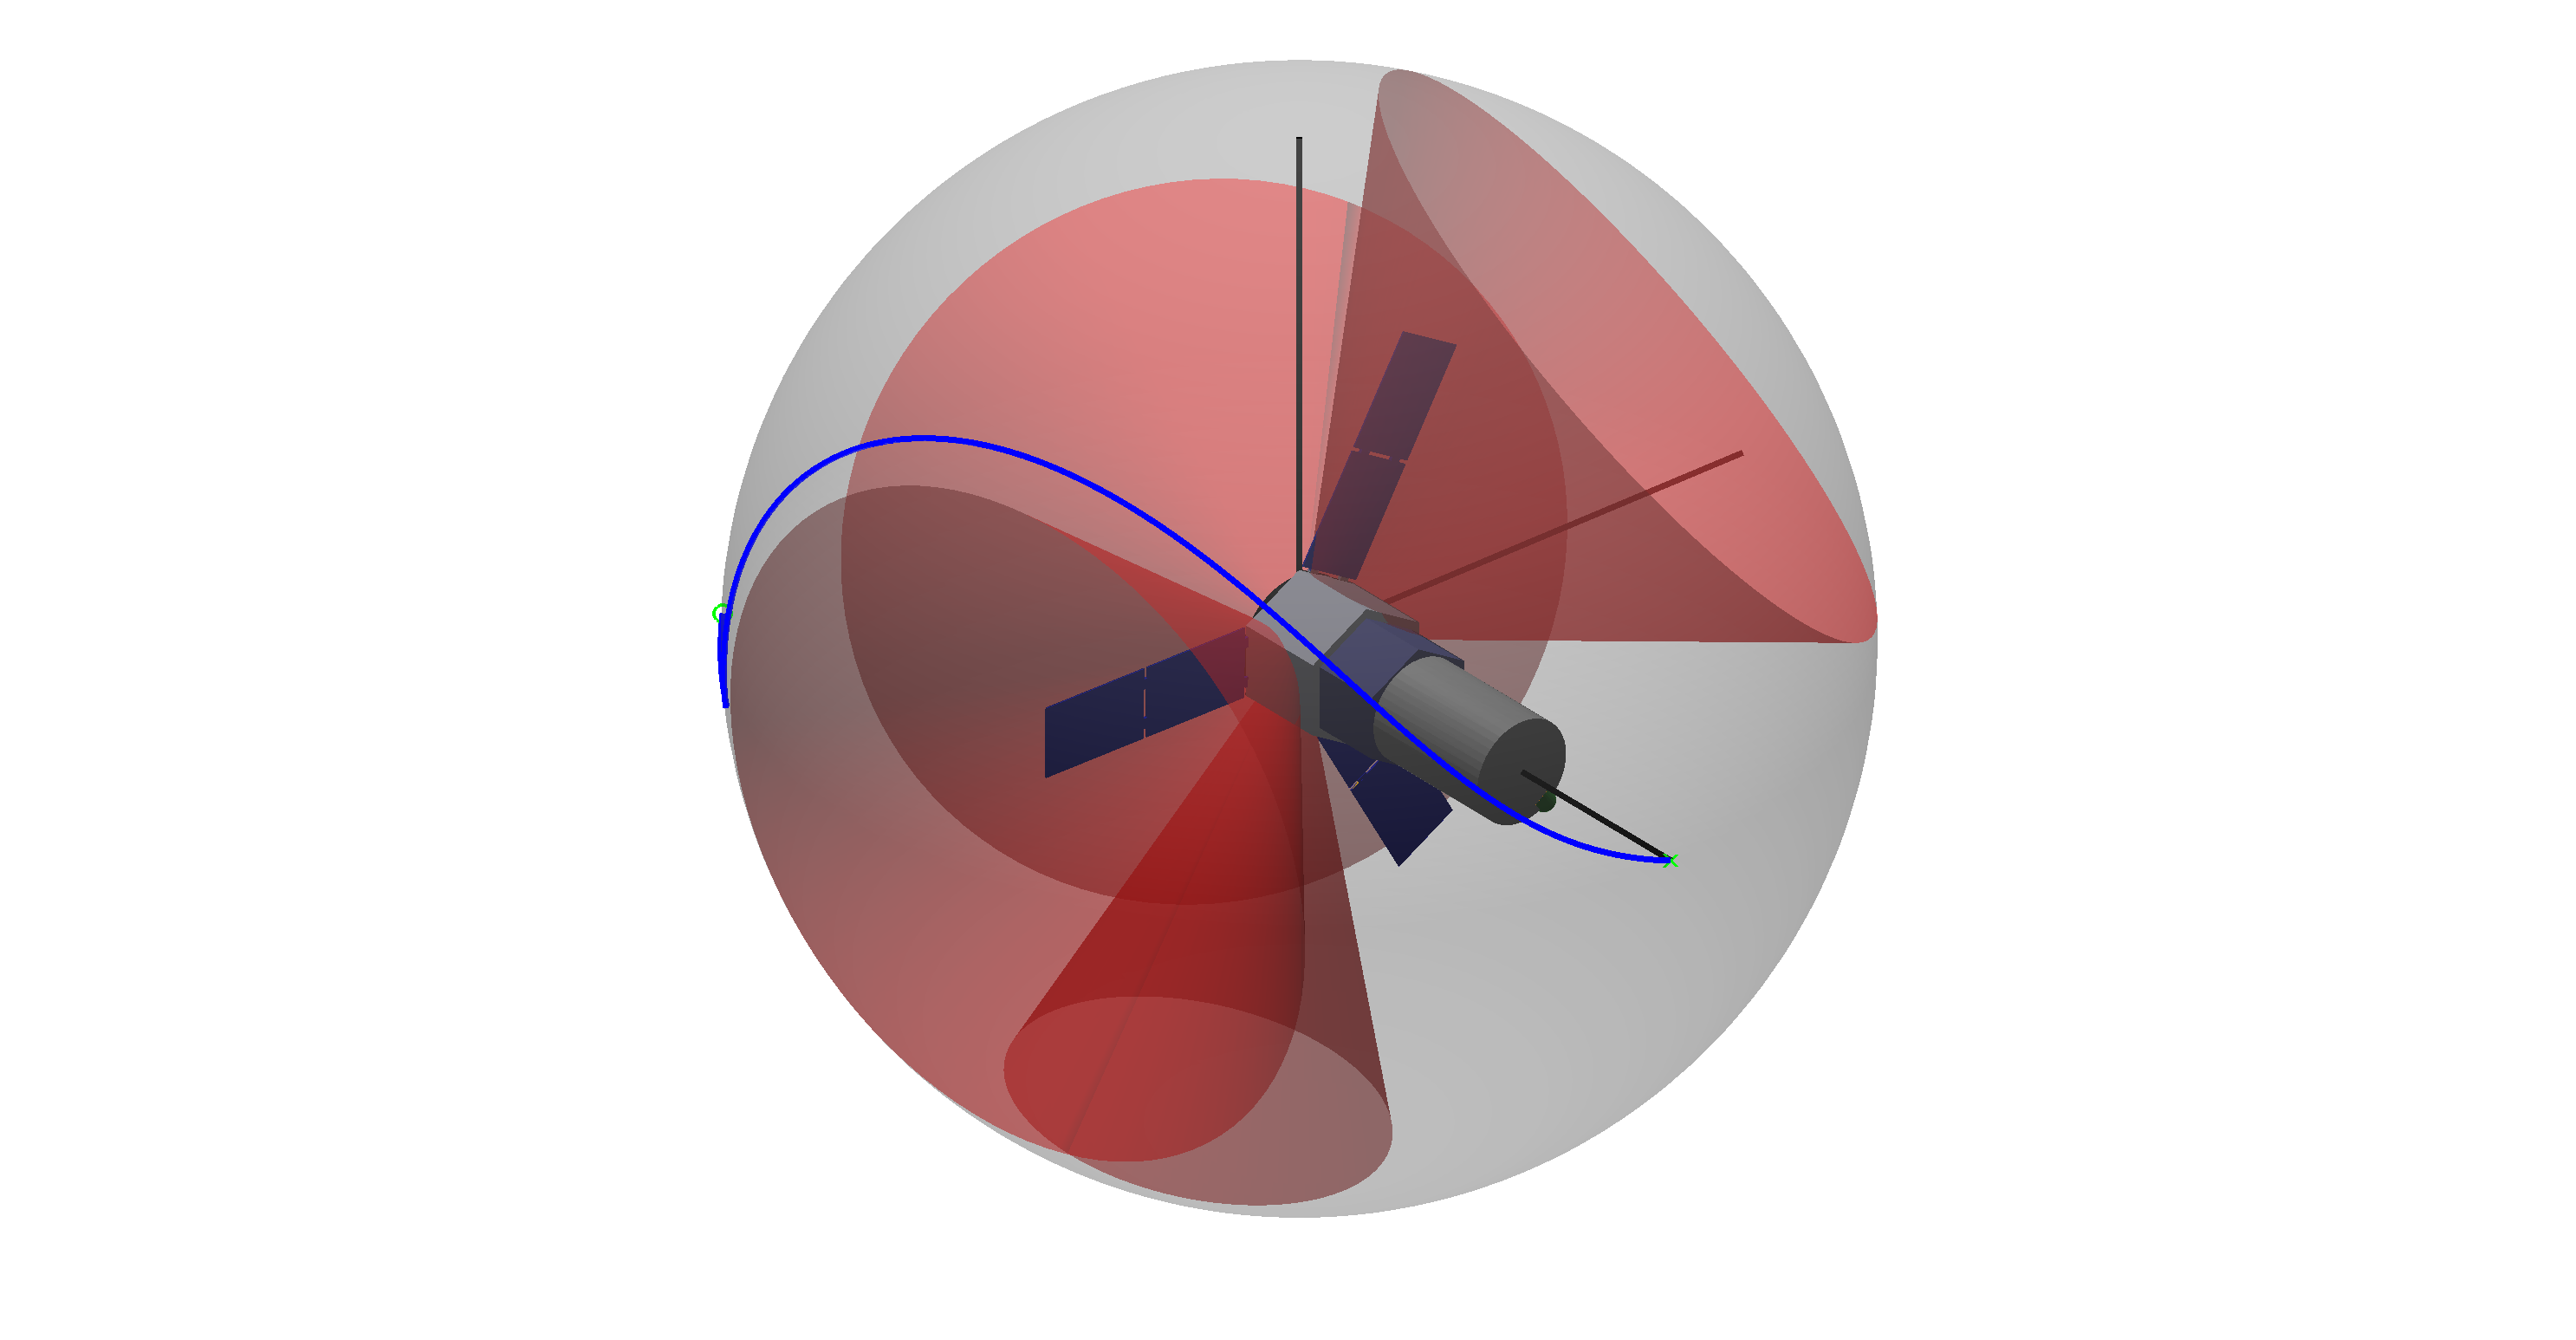
\includegraphics[trim={10cm 0 10cm 0},clip,width=0.75\textwidth]{figures/2016_IJCAS/cad_adapt}
    \caption{Attitude stabilization with adaptive update law trajectory.\label{fig:cad_adapt}}
\end{figure}
The control system is able to asymptotically converge to the desired attitude.
\Cref{fig:con_angles} shows that the angle, \( \arccos(r^T R^T v_i) \) and measured in degrees, between the body fixed sensor and each constraint is satisfied for the entire maneuver.
In addition, the estimate of the disturbance converges to the true value as shown in~\cref{fig:delta_adapt}.

Both control system are able to automatically avoid the constrained regions. 
In addition, these results show that it is straightforward to incorporate an arbitrary amount of large constraints.
In spite of this challenging configuration space, the proposed control system offers a simple method of avoiding constrained regions.
These closed-loop feedback results are computed in real time and offer a significant advantage over typical open-loop planning methods.
These results show that the proposed geometric adaptive approach is critical to attitude stabilization in the presence of state constraints and disturbances.

\paragraph{Time-varying Disturbance}\label{ssec:time_varying}

The form of the uncertainty, given in~\cref{eq:Wdot}, is commonly used in the adaptive control literature~\cite{lee2011a,ioannou2012}. 
A wide variety of realistic disturbances, such as gravitational gradients or malfunctioning thrusters for spacecraft scenarios, are accurately represented via this model. 
In addition, it is possible to represent the uncertainty of a time-varying inertia matrix as an equivalent external disturbance. 
For example, Euler's law gives the relationship for the rate of change of angular momentum as
\begin{align*}
    M_{ext} = \dot{\vc{H}} = \dot{J} \vc{\Omega} + J \dot{\vc{\Omega}} .
\end{align*}
Using this, we can see that an instantaneous change in \( J \) is proportional to an external moment.
Finally, it has been shown that this adaptive control formulation is able to handle time-varying disturbances under some mild assumptions~\cite{ioannou2012}. 

We demonstrate the ability to handle an uncertain time-varying disturbance via numerical example.
The system is identical to the one presented in~\Cref{sec:constrained_attitude_control_numerical_example}, however we modify the external disturbance. 
The external disturbance is the superposition of constant and time-varying terms as
\begin{align*}
    \Delta = \begin{bmatrix} 0.2 \\ 0.2 \\0.2 \end{bmatrix} + 0.02 \begin{bmatrix} \sin 9 t \\ \cos 9 t \\ \frac{1}{2} \parenth{\sin 9t + \cos 9t}\end{bmatrix} \si{\newton\meter}.
\end{align*}
We define a constraint in the inertial frame as \( v = [\frac{1}{\sqrt{2}}, \frac{1}{\sqrt{2}}, 0]^T \) with \( \theta = \ang{12} \).
The initial state is defined as \(R(0) = \exp( \frac{\pi}{2} \hat{e}_3) \), while the desired state is \(R_d =I \).
The goal is to rotate the vehicle about the \( e_3 \) axis while avoiding the obstacle and compensating for the time-varying disturbance. 

\begin{figure}[htbp]
    \centering
    \begin{tikzpicture}[baseline]
    \begin{axis}[
        name={Psi_timevarying},
        ylabel={$\Psi$},
        xlabel={$t~(\si{\second})$},
        ]
        \addplot [blue, mark=none] table [x=TIME, y=Psi, col sep=comma] {figures/2016_IJCAS_pgf/csv/timevarying.csv};
        \addplot [red, mark=none, dashed] coordinates {
                (0.0, 0.0) (10.0, 0.0) 
            };
    \end{axis}
\end{tikzpicture}

    \caption{Configuration error \( \Psi \) for attitude control with adaptive update law assuming a time varying external disturbance.
    The desired attitude corresponding to \( \Psi = 0 \) is denoted in red.\label{fig:Psi_tv}}
\end{figure}
\Cref{fig:Psi_tv,fig:con_angle_tv,fig:Delta_tv} demonstrates the ability for the adaptive controller, which is presented in~\Cref{prop:adaptive_control}, to handle time-varying disturbances.
\Cref{fig:Psi_tv} shows the non-dimensional value of the configuration error function and demonstrates that the adaptive controller is able to stabilize the system to the desired attitude configuration.
In addition,~\cref{fig:con_angle_tv} shows that the constraint is never violated as the angle between the body-fixed sensor \( r \) and the constraint \( v \) is greater than \SI{12}{\degree} over the entire attitude maneuver.
\begin{figure}[htbp]
    \centering
    \begin{tikzpicture}
    \begin{axis}[
        name={ang_con_timevarying},
        ylabel={ $\arccos \parenth{r^T R^T v_i}$},
        xlabel={$t~(\si{\second})$},
        ]
        \addplot +[mark=none] table [x=TIME, y=ang_con, col sep=comma] {figures/2016_IJCAS_pgf/csv/timevarying.csv}; 
    \end{axis} 
\end{tikzpicture}

    \caption{Angle between the sensor view axis and the constraint for attitude control with adaptive update law with a time varying disturbance. \label{fig:con_angle_tv}}
\end{figure}
We can see in~\cref{fig:Delta_tv} that that estimate \(\bar \Delta \) for each of the components accurately tracks the true disturbance after approximately~\SI{5}{\second}.
\begin{figure}[htbp]
    \centering
    \tikzsetnextfilename{dist_timevarying}
\begin{tikzpicture}[]
    \begin{groupplot}[
        group style={
            group name={dist_timevarying},
            group size=1 by 3,
            xlabels at=edge bottom,
            ylabels at=edge left,
            xticklabels at=edge bottom,
            vertical sep=0pt,
        },
        xlabel={$t~(\si{\second})$},
        width=0.8\textwidth,
        height=0.2\textheight,
        scale only axis,
    ]
    \nextgroupplot[ylabel={$ \Delta_1 $}]
    \addplot [ultra thick, blue, mark=none] table [x=TIME, y=D_1, col sep=comma] {figures/2016_IJCAS_pgf/csv/timevarying.csv};
    \addplot [ultra thick, red, mark=none, dashed] table [x=TIME, y=D_true_1, col sep=comma] {figures/2016_IJCAS_pgf/csv/timevarying.csv};

    \nextgroupplot[ylabel={$ \Delta_2 $}]
    \addplot [ultra thick, blue, mark=none] table [x=TIME, y=D_2, col sep=comma] {figures/2016_IJCAS_pgf/csv/timevarying.csv};
    \addplot [ultra thick, red, mark=none, dashed] table [x=TIME, y=D_true_2, col sep=comma] {figures/2016_IJCAS_pgf/csv/timevarying.csv};

    \nextgroupplot[ylabel={$ \Delta_3 $}]
    \addplot [ultra thick, blue, mark=none] table [x=TIME, y=D_3, col sep=comma] {figures/2016_IJCAS_pgf/csv/timevarying.csv};
    \addplot [ultra thick, red, mark=none, dashed] table [x=TIME, y=D_true_3, col sep=comma] {figures/2016_IJCAS_pgf/csv/timevarying.csv};
\end{groupplot}
\end{tikzpicture}

    \caption{Distance estimate \( \Delta \) components for attitude control with adaptive update law and time varying disturbance.
    The controller is able to accurately estimate the varying disturbance\label{fig:Delta_tv}}
\end{figure}

\section{Experiment on Hexrotor UAV}\label{sec:experiment}

\begin{figure}[htbp]
    \centering
    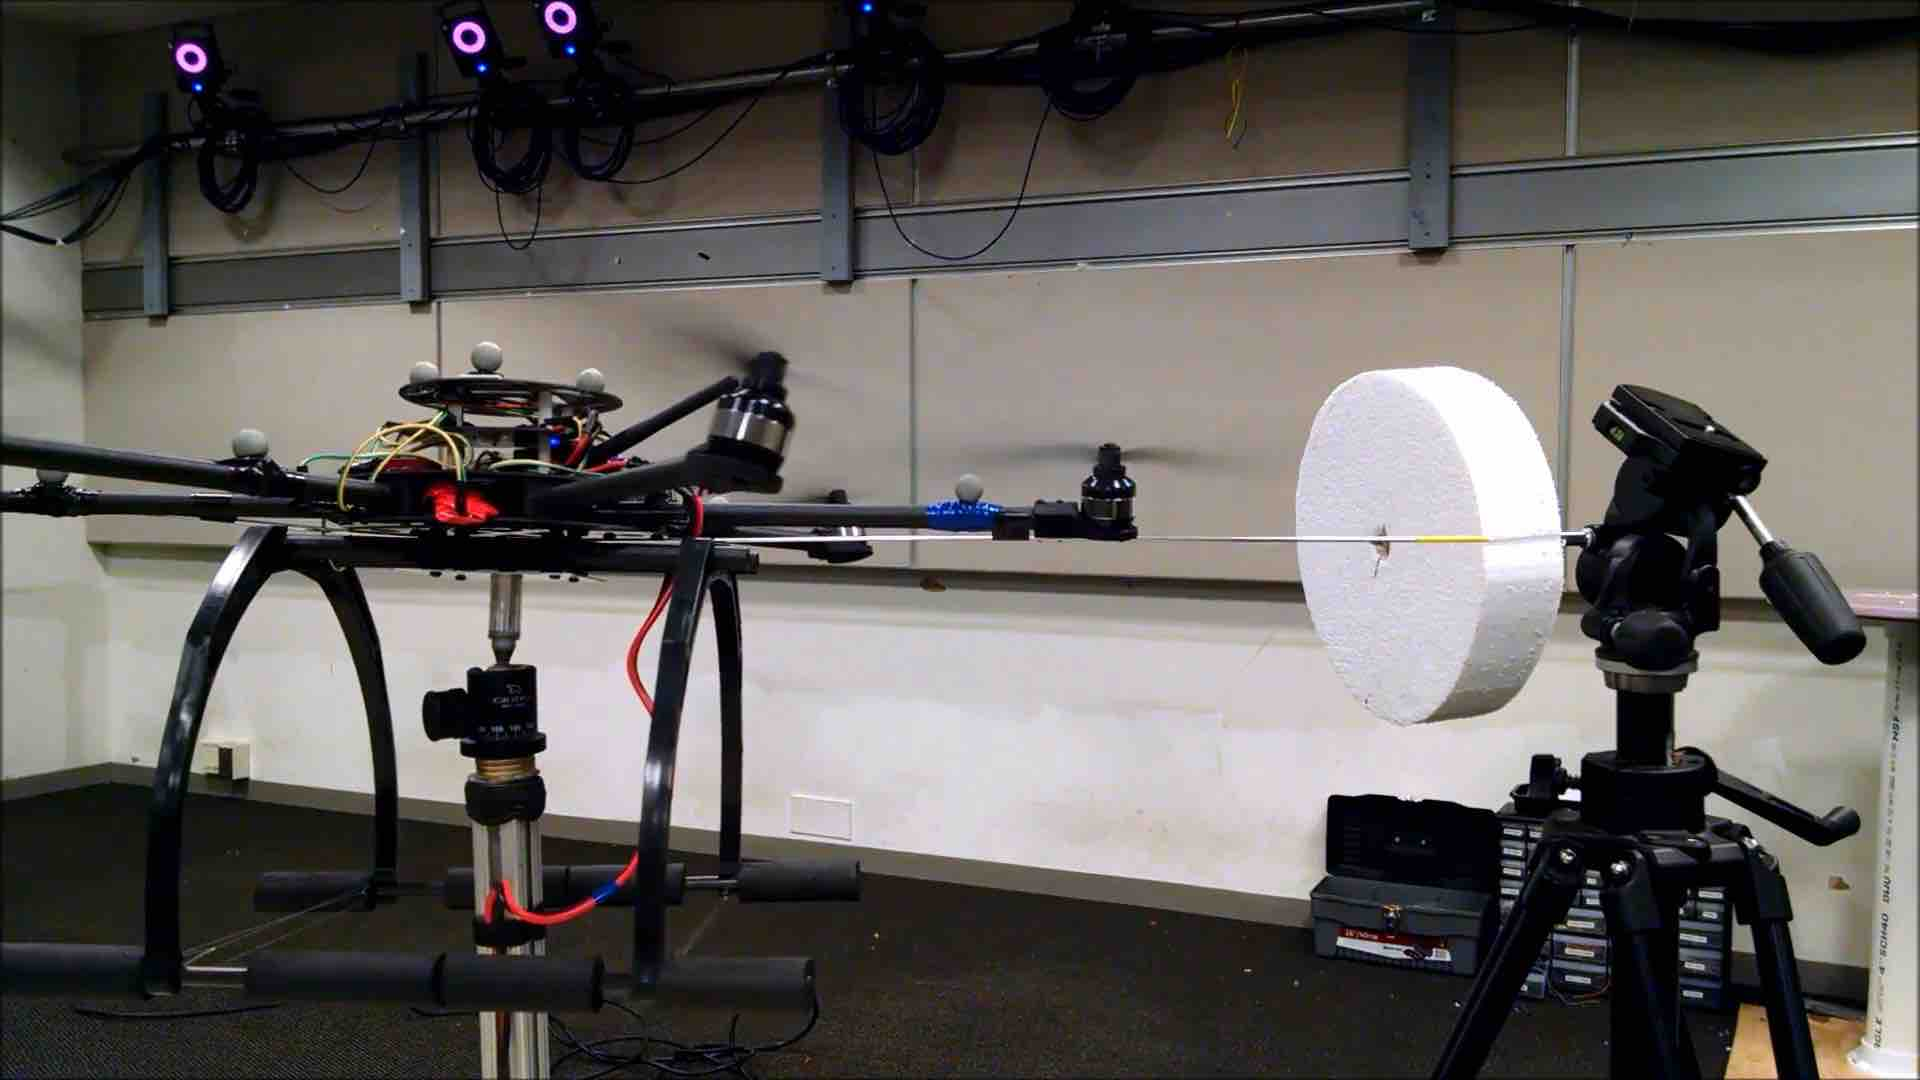
\includegraphics[width = 0.7\columnwidth]{2016_IJCAS/hexrotor}
    \caption{Attitude control testbed~\label{fig:hexrotor}}
\end{figure}
\vspace{-3mm}
A hexrotor unmanned aerial vehicle (UAV), as seen in~\cref{fig:hexrotor}, has been developed at the Flight Dynamics and Controls Laboratory (FDCL) at the George Washington University.
The UAV is composed of three pairs of counter-rotating propellers. 
Typical UAVs are composed of four or more co-planar propellers.
As a result, these systems are underactuated and unable to impart a force along every degree of freedom.
For example, quadrotor UAVs are unable to translate laterally without first conducting a rotation.
Conversely, the propeller pairs of the hexrotor are angled relative to one another to allow for a fully actuated rigid body.
This allows the hexrotor to impart a force in any direction and a moment about any axis. 

Attitude information is measured by a combination of both on and off board sensor systems.
The VectorNav VN-100 is a rugged, miniature high-performance inertial measurement unit which provides high frequency angular velocity measurements.
A Vicon motion capture system is installed within the test environment and used to provide high accuracy attitude measurements. 
A series of reflective markers are placed on the hexrotor and their relative position is captured by a series of infrared optical cameras. 
Assuming a fixed rigid body, the Vicon system is able to derive the attitude of the hexrotor and transmit this data to the processor onboard the hexrotor.
The control input is computed on-board, using the full state measurement, and implemented at approximately \SI{100}{\hertz}.
In order to constrain the motion, allowing us to test only the attitude dynamics, we attach the hexrotor to a spherical joint.
Since, the center of rotation is below the center of gravity of the hexrotor there is a destabilizing gravitational moment.
The resulting attitude dynamics are similar to an inverted pendulum model.
We augment the control input in~\cref{eqn:adaptive_control} with an additional term to negate the effect of the gravitational moment.

A sensor pointing direction is defined in the body-fixed frame of the hexrotor as \( r = [1,0,0]^T \).
We define an obstacle in the inertial frame as \( v = [\frac{1}{\sqrt{2}}, \frac{1}{\sqrt{2}}, 0]^T \) with \( \theta = \ang{12} \).
An initial state is defined as \(R(0) = \exp( \frac{\pi}{2} \hat{e}_3) \), while the desired state is \(R_d =I \).
This results in the UAV performing a \ang{90} yaw rotation about the vertical axis of the spherical joint and the constrained region is on the shortest path connecting $R_0$ and $R_d$. 
The attitude control system is identical to the one presented in~\Cref{prop:adaptive_control} with the exception of a gravity moment term, \( M_g = r_{cg} \times m g R^T e_3\) which represents the gravitational moment due to the distance \( r_{cg} \) between the center of mass and the center of rotation. 
In addition, the following parameters were also modified: \(k_R = 0.4, k_\Omega = 0.7 ,c = 0.1 , \alpha = 8 \text{ and } k_\Delta = 0.05\) to account for the differences in the hardware model of the hexrotor.
\begin{figure}[t]
    \centering 
    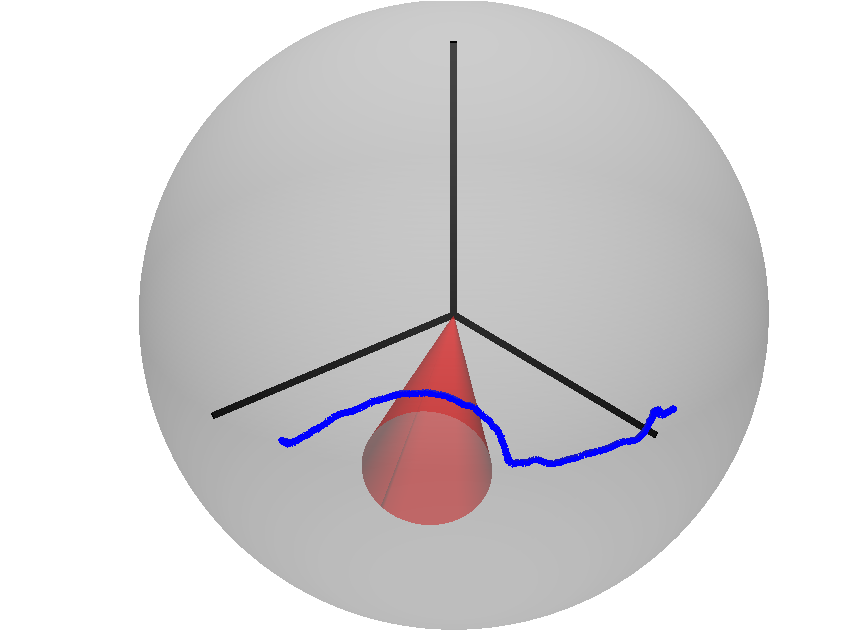
\includegraphics[width=0.75\columnwidth]{2016_IJCAS/traj_exp}
    \caption{ Attitude trajectory for hexrotor experiment.\label{fig:traj_exp} }
    \label{fig:exp} 
\end{figure}

The experimental results are shown in~\Cref{fig:exp}.
\Cref{fig:eR_exp,fig:Psi_adapt,fig:eR_exp,fig:u_exp,fig:con_angle_exp} shows the behavior of each of the components of the attitude error vector, defined by~\cref{eq:eR}, over the experiment time span.
\begin{figure}[htbp]
    \centering
    \tikzsetnextfilename{eR_exp}
\begin{tikzpicture}[baseline]
    \begin{groupplot}[
        group style={
            group name={eR_exp},
            group size=1 by 3,
            xlabels at=edge bottom,
            ylabels at=edge left,
            xticklabels at=edge bottom,
            vertical sep=0pt,
        },
        xlabel={$t~(\si{\second})$},
        ymin=-1.5, ymax=1.5,
        scale only axis,
        width=0.8\textwidth,
        height=0.1\textheight,
    ]
    \nextgroupplot[ylabel={$ e_{R_1}$}]
    \addplot [ultra thick,blue, mark=none] table [x=TIME, y=eR_1, col sep=comma] {figures/2016_IJCAS_pgf/csv/exp.csv};
    \addplot [ultra thick,red, mark=none, dashed] coordinates {
        (0.0, 0.0) (12.0, 0.0) 
    };
    \nextgroupplot[ylabel={$ e_{R_2}$}]
        \addplot [ultra thick,blue, mark=none] table [x=TIME, y=eR_2, col sep=comma] {figures/2016_IJCAS_pgf/csv/exp.csv};
        \addplot [ultra thick,red, mark=none, dashed] coordinates {
            (0.0, 0.0) (12.0, 0.0) 
        };
    \nextgroupplot[ylabel={$ e_{R_3}$}]
        \addplot [ultra thick,blue, mark=non] table [x=TIME, y=eR_3, col sep=comma] {figures/2016_IJCAS_pgf/csv/exp.csv};
        \addplot [ultra thick,red, mark=none, dashed] coordinates {
            (0.0, 0.0) (12.0, 0.0) 
        };
\end{groupplot}
\end{tikzpicture}

    \caption{Attitude error vector \( e_R \) components for hexrotor experiment.
    The desired attitude corresponding to \( e_R = 0 \) is denoted in red.\label{fig:eR_exp}}
\end{figure}
\Cref{fig:Psi_exp} shows the time history of the attitude error function, defined by~\cref{eq:psi}.
\begin{figure}[htbp]
    \centering
    \tikzsetnextfilename{Psi_exp}
\begin{tikzpicture}[baseline]
    \begin{axis}[
        name={Psi_exp},
        ylabel={$\Psi$},
        xlabel={$t~(\si{\second})$},
        scale only axis,
        width=0.8\textwidth,
        height=0.2\textheight,
        ]
        \addplot [ultra thick,blue, mark=none] table [x=TIME, y=Psi, col sep=comma] {figures/2016_IJCAS_pgf/csv/exp.csv};
        \addplot [ultra thick,red, mark=none, dashed] coordinates {
                (0.0, 0.0) (12.0, 0.0) 
            };
    \end{axis}
\end{tikzpicture}

    \caption{Configuration error \( \Psi \) for hexrotor experiment.
    The desired attitude corresponding to \( \Psi = 0 \) is denoted in red.\label{fig:Psi_exp}}
\end{figure}
\Cref{fig:u_exp} shows the magnitude of each component of the control input in \si{\newton\meter}, which is computed from~\cref{eqn:adaptive_control}.
Finally,~\cref{fig:con_angle_exp} shows the angle between the body-fixed sensor and the obstacle in degrees.
\begin{figure}[htbp]
    \centering
    \tikzsetnextfilename{u_exp}
\begin{tikzpicture}[baseline]
    \begin{groupplot}[
        group style={
            group name={u_exp},
            group size=1 by 3,
            xlabels at=edge bottom,
            ylabels at=edge left,
            xticklabels at=edge bottom,
            vertical sep=0pt,
        },
        xlabel={$t~(\si{\second})$},
        ymin=-1.5, ymax=1.5,
        scale only axis,
        width=0.8\textwidth,
        height=0.1\textheight,
    ]
    \nextgroupplot[ylabel={$ u_1 $}]
    \addplot [ultra thick, blue, mark=none] table [x=TIME, y=u_1, col sep=comma] {figures/2016_IJCAS_pgf/csv/exp.csv};
    \addplot [ultra thick, red, mark=none, dashed] coordinates {
        (0.0, 0.0) (12.0, 0.0) 
    };
    \nextgroupplot[ylabel={$ u_2 $}]
        \addplot [ultra thick, blue, mark=none] table [x=TIME, y=u_2, col sep=comma] {figures/2016_IJCAS_pgf/csv/exp.csv};
        \addplot [ultra thick, red, mark=none, dashed] coordinates {
            (0.0, 0.0) (12.0, 0.0) 
        };
    \nextgroupplot[ylabel={$ u_3 $}]
        \addplot [ultra thick, blue, mark=non] table [x=TIME, y=u_3, col sep=comma] {figures/2016_IJCAS_pgf/csv/exp.csv};
        \addplot [ultra thick, red, mark=none, dashed] coordinates {
            (0.0, 0.0) (12.0, 0.0) 
        };
\end{groupplot}
\end{tikzpicture}

    \caption{Control input \( u \) components for hexrotor experiment.\label{fig:u_exp}}
\end{figure}
In order to maneuver the system ``close'' to the constrained zone we utilize several intermediary set points on either side of the obstacle.
From the initial attitude the hexrotor rotates to the first set point, pauses, and then continues around the obstacle to the second set point before continuing toward the desired attitude.
As a result this creates the stepped behavior of the configuration error history as shown in~\cref{fig:Psi_exp}.
\begin{figure}[htbp]
    \centering
    \tikzsetnextfilename{ang_con_exp}
\begin{tikzpicture}
    \begin{axis}[
        name={ang_con_exp},
        ylabel={ $\arccos \parenth{r^T R^T v_i}$},
        xlabel={$t~(\si{\second})$},
        ]
        \addplot +[mark=none] table [x=TIME, y=ang_con, col sep=comma] {figures/2016_IJCAS_pgf/csv/exp.csv}; 
    \end{axis} 
\end{tikzpicture}

    \caption{Angle between the sensor view axis and the constraint for hexrotor experiment.
    The attitude controller is able to satisfy the constraint. \label{fig:con_angle_exp}}
\end{figure}

The hexrotor avoids the constrained region illustrated by the circular cone in \cref{fig:traj_exp}, by rotating around the boundary of the constraint. 
\Cref{fig:con_angle_exp} shows the angle, \( \arccos \parenth{r^T R^T v} \), between the body mounted sensor and the inertially fixed sensor.
The experiment demonstrates that the minimum angular separation is \SI{14}{\degree} which satisfies the constraint of \( \theta = \SI{12}{\degree} \).
This further validates that the proposed control system exhibits the desired performance in the experimental setting as well. 
A video clip is available at \url{https://youtu.be/dsmAbwQram4}.

\section{Summary}

This section presented the nonlinear geometric control of a rigid body around a small body.
The controllers are derived on the special euclidean group and avoid the issues inherent in parameterizing motion in the form of local coordinates.
In addition, a new adaptive attitude control for state inequality constraints is developed.
This enables the accurate stabilization and tracking of a desired attitude while avoiding obstacles.

The control approaches presented in this chapter, when combined with the results of~\cref{sec:lowthrust_transfers}, provide a complete approach for the manuevering of a spacecraft around a small body. 
The low thrust propulsion scheme of~\cref{sec:lowthrust_transfers} is ideal for large magnitude orbital changes, while the results of this chapter provide precise trajectory tracking ideal for low altitude operations.
These nonlinear controllers are ideally suited for low altitude operations.
The results are utilized in the subsequent chapters to explore an asteroid and land on the surface.
